\documentclass[11pt,a4paper,twoside]{article}
\usepackage[top=70pt,bottom=80pt,left=78pt,right=76pt]{geometry}
\usepackage[utf8]{inputenc}
\usepackage[english]{babel}
% \selectlanguage{english}
\usepackage[T1]{fontenc}
\usepackage{lmodern}
% \usepackage{booktabs}
\usepackage{ctable}
\usepackage{graphicx}
\graphicspath{{./images/}}
\usepackage{subfig}
\usepackage{longtable}
\usepackage{amsmath, amssymb}
\usepackage{natbib, url}
\usepackage[chapter, nottoc]{tocbibind} % Fix heading in bibs etc
\usepackage{array}
\usepackage{float}
\usepackage{caption}
% \usepackage{subcaption}
\usepackage{epstopdf}
% \usepackage{gensymb}
\usepackage{listings}
\newcommand*\PBS[1]{\let\temp=\\#1\let\\=\temp}

\begin{document}

\newlength{\figurewidth}\setlength{\figurewidth}{0.95\textwidth}
\begin{titlepage}
  \begin{center}

% 	\includegraphics[width=4cm]{LogoEng}
    % \vspace{1.5cm}

    \begin{LARGE}
      \bfseries
      Victors Thesis - Title could be improved\\
    \end{LARGE}

    \vspace{1cm}

    \begin{Large}
      \bfseries
       Victor Öhman\\[1ex]
    \end{Large}

    \vspace{1cm}
    \vspace{1.5cm}
    \begin{small}
      Division of Fluid Dynamics\\
			Department of Management and Engineering\\
      Linköpings Universitetet\\
      SE-581 83 Linköping, Sweden\\

    \end{small}
    \vspace{1cm}
    % \rule{\textwidth}{0.1mm}
     \vspace{0.5cm}
		 \begin{small}
      \bfseries
    \end{small}
	\end{center}
\end{titlepage}
\raggedbottom
\thispagestyle{empty}
\cleardoublepage

%\frontmatter

\pagenumbering{roman}
\section*{Abstract} %informative (not descriptive)

Lorem ipsum dolor sit amet, consectetur adipiscing elit. Integer euismod interdum diam, eu lobortis libero bibendum in. Vestibulum molestie aliquam ante. Morbi in tortor eu arcu fermentum maximus. Etiam egestas fringilla interdum. Nunc non ullamcorper turpis, eu cursus ipsum. Nulla suscipit tristique nisi id consequat. Donec tellus ligula, feugiat id cursus at, bibendum at velit.

\clearpage
\thispagestyle{empty}
\cleardoublepage
\thispagestyle{plain}


\section*{Acknowledgments}

Lorem ipsum dolor sit amet, consectetur adipiscing elit. Integer euismod interdum diam, eu lobortis libero bibendum in. Vestibulum molestie aliquam ante. Morbi in tortor eu arcu fermentum maximus. Etiam egestas fringilla interdum. Nunc non ullamcorper turpis, eu cursus ipsum. Nulla suscipit tristique nisi id consequat. Donec tellus ligula, feugiat id cursus at, bibendum at velit.

\clearpage
\thispagestyle{empty}
\cleardoublepage
\thispagestyle{plain}


\section*{Notational Conventions}
\label{cha:notation}
\vspace{-2ex}


\section*{Abbreviations and Acronyms}
\vspace*{-2ex}
\begin{longtable}{p{.25\textwidth}p{.65\textwidth}} % Abbreviations

 \multicolumn{1}{l}{\bfseries Abbreviation} &
 \multicolumn{1}{l}{\bfseries Meaning}\\

\endhead
\endfoot

LiU     & Linköping University\\
LiTH	  & Linköpings tekniska högskola \\
DoF		  & Degrees of Freedom \\
CAD     & Computer aided design\\
PWM     & Pulse-width Modulation\\

\end{longtable}
\vspace*{1ex}


\section*{Symbols and Mathematical Notation}
\vspace*{-2ex}
\setlength\extrarowheight{1pt}
\begin{longtable}{>{$\displaystyle}p{.25\textwidth}<{$}p{.65\textwidth}} % Math
  \multicolumn{1}{l}{\bfseries Notation} &
  \multicolumn{1}{l}{\bfseries Meaning}\\
\endhead
\endfoot
a 												& Small letter\\
C_{D} 										& Large letter\\
\vec n 										& Normal vector\\
p 												& Pressure\\
t 												& Time\\
\alpha 										& Angle\\
\end{longtable}


\clearpage
\thispagestyle{empty}
\cleardoublepage
\tableofcontents

\clearpage
\thispagestyle{empty}
\listoffigures

\clearpage
\thispagestyle{empty}
\listoftables

\clearpage
\thispagestyle{empty}
%\mainmatter
\pagenumbering{arabic}


\newpage
\section{Introduction}

\subsection{Background}
\subsection{Thesis Outline}

Coc

From this part in the report existing subsystems in the model are addressed with a bold typeface.
 %
% mentions matlab, how spell, how ref? change accordingly in text
\subsection{Frame of Reference}

The model built in this thesis is being built in Matlab and SIMULINK with the tools from the aerospace toolbox. Important to note is that the aerospace blockset sold by mathworks is not used here. At the time of writing no student license used did not include the aerospace blockset, and as others might be in the same position, the simulation model is completed without the blockset. 

       % "CHAPTER" 1
\section{Aircraft Model Overview}

\subsection{Blocks \& Definitions}

This part contains a summary of some of the commonly used blocks in the model along with the function and some specific properties not explained elsewhere.

% What is missing from here?
% Delimitations?
 % maybe common + pictured
\subsection{General Model Outline}

A visual representation of the model is shown below in figure \ref{fig:schematic-modeloutline}. This interpretation of the system contains the most important areas and how they depend on eachother for information. This will make it easier to inspect these areas in detail as we go along.

%%%%%%%%%%%%%%%%%%%%%%%%%%%%%%%%%%%%%%%%%%%%
%                                          %
%                                          %
%                                          %
%                                          %
%                                          %
%                                          %
%       fig:schematic-modeloutline         %
%                                          % Shade code along control
%                                          % and flight data
%                                          %
%                                          %
%                                          %
%                                          %
%                                          %
%%%%%%%%%%%%%%%%%%%%%%%%%%%%%%%%%%%%%%%%%%%%

Since the model should be able to make use of live input from a pilot as well as actual flight data from a timeseries, the schematic is shaded along the logical path of using recorded flight data. The parts of certain interest that are explained further into the report are represented in the list as follows.

\begin{itemize}
  \item Pilot Control
    \begin{itemize}
      \item Flight Data
      \item Live Flight
    \end{itemize}
  \item Engine
  \item Aerodynamics
  \begin{itemize}
    \item Flight Data
    \item Live Flight
  \end{itemize}
  \item Dynamics
  \begin{itemize}
    \item 3DoF for Longitudinal Stability
    \item 6DoF Complete Model
  \end{itemize}
  \item Visualization
  \item Environment
\end{itemize}

The part using 3DoF while being important is in essense a tool used for the purpose of investigating longitudinal stability before connecting the 6DoF to also assess lateral stability. It is thus a included in the part explaining the 6DoF model and does not need to be explained separately.

% What is missing from here?
% Delimitations?
 % showing nice looking schematic
         % "CHAPTER" 2
\newpage
\section{Aircraft Model Interioir}

% UNDONE
\subsection{Aircraft Flight Dynamics}

%The fourth and last major part in the top level of the model is the aircraft dynamics part.

The subsystem called \textsc{Dynamics} takes the input in terms of forces and moments and outputs the so called \textit{Plant Data} which is then used throughout the model and could be looked at as the current state of the model for the coming timestep. The data collected in \textit{Plant Data} is explained later.

% v1
% Missing LLA (how ned it?)
% Eq undone
% abbrev NED
% missing image
% 1 delim
% use word cartesian somehwere, maybe euler too?
\subsubsection{Inertial Reference Frame}

In simple terms, two axis systems are needed to build an aircraft model (and the majority of models with moving parts as well for that matter), one that is fixed and decides where the origin is located and one that is attached to the moving body. In this project the fixed reference frame, \textbf{$X_e$}, is a vector composed of the position in the x direction $X^e$, the position in the y-direction $Y^e$ and the altitude of the aircraft in the z-direction $Z^e$. The practical use for these values in the model is to declare them as the initial values for each and any simulation, hence, these values are found as follows.

%\begin{equation}
% nonumber Xe => Xe_0
% nonumber Ye => Ye_0
% nonumber Z_e => $h\_{ini}$
%\end{equation}

%%%%%%%%%%%%%% IMAGE OF FIXED AND BODY AND LINE BETWEEN

%
% Delimitation
%
To make use of Newton's laws an intertial frame has to be defined. In this project the earth's surface is assumed flat and non-rotating.
%

To know which way the frame should be positioned a \textsc{NED, North, East, Down} system is used, making the positive x-axis directed North, the positive y-axis directed East and the positive z-axis directed down towards the surface of the earth with the origin in the moving body. These are the values that are used as the output position in every timestep of the simulation.

% v1
% abbrev CG, Vb, AC (undeclared in text), \alpha
% stab?
% use word cartesian somehwere, maybe euler too?
\subsubsection{Body \& Wind Frame}

The AC body frame is an axis system with the origin located at the CG of the body, the positive x-axis parallel to fuselage forward axis in the aircraft body, the positive y-axis on the right hand side of the pilot (starboard) and the positive z-axis directed down towards the ground. A vector, \textbf{$V_b$}, consisting of $V^b_x$, $V^b_y$ and $V^b_z$ constitutes the body velocity in these directions and can be seen as a vector of projections of the relative wind on the body axes. The rotations along each axis are the Euler rotation angles $\phi$ for roll around the x-axis, $\theta$ for pitch around the y-axis and $\psi$ for heading rotation around the z-axis. Figure \ref{BodyWindFrameRot}

% IMAGE
\label{BodyWindFrameRot}

The body frame is rotated with a \textsc{DCM, Directional Cosine Matrix}
% this needs to be filled out, this is with regard to euler angles, alpha and beta can be described more in aerodynamics
The wind frame, with vector named \textbf{$V_w$} is a lot like the body frame, but has the x-axis directed along the actual flight path. In practice this is the calculated airspeed of the aircraft as the first component of the vector, with the projections of the second and third component at zero. The airspeed from this point will be called V.

% show V_w in a vector with the projections (if I didnt brainfart here) 

As output values the body velocity \textbf{$V_b$} represents the translational characteristics over the timesteps with

\subsubsection{Equations of Motion}

\subsubsection{Longitudinal Stability}
\subsubsection{Lateral Stability}



% Explain plant data
% What is missing from here?
% Delimitations?


\subsection{Aerodynamic \& Engine Forces}

The forces and moments section is devoted to the largest parts primaliry giving output in forces and moments. These are the \textbf{Engine} subsystem and the \textbf{Aerodynamics} subsystem, and they are described below in this order.

\subsubsection{Engine System}

The engine system is a subsystem accessible form the top level of the overall system, right next to the aerodynamics system, and is built to take the throttle command, the nozzle pitch command and the nozzle yaw command from the \textbf{Control} subsystem and to output forces and moments generated by the propulsion in effect.

% Add some talk about details like
% 1/0 throttle
% damping
% nozzle and angles, pictures for ease, equations too

\subsubsection{Aerodynamics}

A first aerodynamic model is built. It is however missing some parts so far.


% What is missing from here?
% Delimitations?
 % aerodynamics and propulsion
 % engine prop, weight, aero



\subsection{Pilot Control	 \& Actuators}

\subsubsection{Pilot \& Control}

The part of the system named \textbf{Control} is the part of the model where the pilot commands are either created or read, depending on if the model is run with live pilot control or is run with recorded data. The pilot control PWM signals (Pulse-Width Modulation) are the command signals representing specific SI values. Values of which they are translated into immediately in the same model block before they are directed into the \textbf{Actuators} subsystem.

\subsubsection{Actuators \& Servos}

The part of the system named \textbf{Actuators} is the part of the model designed to take values from the \textbf{Pilot \& Control} subsystem and run them through the appropriate  output these commands in thrust and control surface deflection angles deflection


% What is missing from here?
% Delimitations?
\subsubsection{Sensors}
 % control and actuator focus


%\subsection{Summary}

% TEST

\begin{table}[H]
\caption{Test table for list of tables.}
\centering
\begin{tabular}{lccr}
 & \textbf{Coarse}& \textbf{Fine} & \textbf{Relative difference} \\
Mesh nodes & 251486 & 569727 & 127\% \\
$C_D$ & 0.05896 & 0.057497 & -2.5\% \\
$C_L$ & 1.3541 & 1.3796 & 1.9\% \\
\end{tabular}
\label{meshilainen3dII}
\end{table}

\begin{figure}[H]
 \centering
 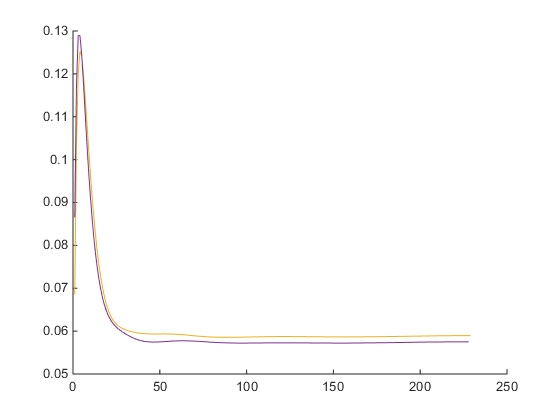
\includegraphics[width=10cm]{TESTimg.png}
 \caption{Test figure for list of figures.}
\label{Cd_mesh_ind}
\end{figure}
 %
         % "CHAPTER" 3
\newpage
\section{Aircraft Model Exterior}

% v1
% delim only logged
% controller 2 l?
\subsection{Pilot}

The pilot input in this project can either be by direct input from a controller or by logged data from an actual flight test with the demonstrator. In this project only logged data from flight tests will be used. The top level subsystem \textbf{Pilot Control} has a manual switch allowing the user to choose between logged data or direct control via controller.

% origin of equations to convert PWM
% introduced \delta_{ca} \delta_{els} \delta_{elp}\delta_{ru} \delta_{T} \delta_{lg}
% need prev talk about base workspace, maybe overall generla somt
\subsubsection{Logged Data}

Leaving the switch to accept data from prerecorded data from pilot control of a flight test with the demonstrator means that all information is taken from a timeseries object. The pilot control data used in this project was saved in a file called \textbf{log_pilotcmd.mat} which is a timeseries object containing 11 values recorded for each timestep during the flight test. The signals are recorded from the controler and are \textit{PWM, Pulse Width Modular} signals.

The signals are taken in by importing the file with the logged data from the base workspace, where it was initially imported as a variable along with the rest of the initial conditions and declared variables and constants. The signals are split two ways, one of which leads to a subsystem that makes use of the signals where the signals are split, using "Demux", and then converted one by one by function blocks according to equations by alejandro???????, giving the deflection angles (\delta_{ca} for canard, \delta_{els} and \delta_{elp} for elevons starboard and port and \delta_{ru} for rudder), thrust (\delta_{T}) from 0 to 1, landing gear (\delta_{lg}) from 0 to 1 and clean pilot controler signals for roll, pitch and yaw. The other subsystem that the signals lead to is one built mainly for testing purposes, where the deflection angles are flat at zero after conversion, the thrust is static and controled by a constant giving out from 0 to 1. The remaining signals are left untouched, since they do not alter the flight anyway.

\subsubsection{Live Piloting}

% Needs updating later
% Talk about the subsystems but really casually, add textsc etc
% Add variables
% Lots of delims here
\subsection{Environment}

The environment system is a simple build since the demonstrator is meant to fly low and with little to no variance in athmosphere. The subsystem as a whole is called environment since it is mostly simple equations and constants with regard to temperature, air density and pressure at ground level. The model takes "Plant Data" as input so subsystems with more complete calculations, like that of athmosphere over different altitude, can be added if needed.

As of now, for subsystems are used. One for terrain, one for wind in the simulated environment, one for ground level athmosphere and one for gravity. The terrain one only includes a statement telling the simulation to stop once the aircraft altitude goes below zero, meaning it has effectively reached the ground.

The wind one is unused as of now.???????

Athmosphere has blablablabla.

Gravity is a vector with the z-axis component assigned the gravitational force imposed by the aircraft body multiplied by $DCM_{be}$, making it a force attached to the body frame easily added elsewhere in the model. 

\subsection{Visuals}




%\input{3generaloutlineext} % showing nice looking schematic
%\subsection{Pilot Control	 \& Actuators}

\subsubsection{Pilot \& Control}

The part of the system named \textbf{Control} is the part of the model where the pilot commands are either created or read, depending on if the model is run with live pilot control or is run with recorded data. The pilot control PWM signals (Pulse-Width Modulation) are the command signals representing specific SI values. Values of which they are translated into immediately in the same model block before they are directed into the \textbf{Actuators} subsystem.

\subsubsection{Actuators \& Servos}

The part of the system named \textbf{Actuators} is the part of the model designed to take values from the \textbf{Pilot \& Control} subsystem and run them through the appropriate  output these commands in thrust and control surface deflection angles deflection


% What is missing from here?
% Delimitations?
\subsubsection{Sensors}
 % control and actuator focus
%\subsection{Aerodynamic \& Engine Forces}

The forces and moments section is devoted to the largest parts primaliry giving output in forces and moments. These are the \textbf{Engine} subsystem and the \textbf{Aerodynamics} subsystem, and they are described below in this order.

\subsubsection{Engine System}

The engine system is a subsystem accessible form the top level of the overall system, right next to the aerodynamics system, and is built to take the throttle command, the nozzle pitch command and the nozzle yaw command from the \textbf{Control} subsystem and to output forces and moments generated by the propulsion in effect.

% Add some talk about details like
% 1/0 throttle
% damping
% nozzle and angles, pictures for ease, equations too

\subsubsection{Aerodynamics}

A first aerodynamic model is built. It is however missing some parts so far.


% What is missing from here?
% Delimitations?
 % aerodynamics and propulsion
 % engine prop, weight, aero
%% UNDONE
\subsection{Aircraft Flight Dynamics}

%The fourth and last major part in the top level of the model is the aircraft dynamics part.

The subsystem called \textsc{Dynamics} takes the input in terms of forces and moments and outputs the so called \textit{Plant Data} which is then used throughout the model and could be looked at as the current state of the model for the coming timestep. The data collected in \textit{Plant Data} is explained later.

% v1
% Missing LLA (how ned it?)
% Eq undone
% abbrev NED
% missing image
% 1 delim
% use word cartesian somehwere, maybe euler too?
\subsubsection{Inertial Reference Frame}

In simple terms, two axis systems are needed to build an aircraft model (and the majority of models with moving parts as well for that matter), one that is fixed and decides where the origin is located and one that is attached to the moving body. In this project the fixed reference frame, \textbf{$X_e$}, is a vector composed of the position in the x direction $X^e$, the position in the y-direction $Y^e$ and the altitude of the aircraft in the z-direction $Z^e$. The practical use for these values in the model is to declare them as the initial values for each and any simulation, hence, these values are found as follows.

%\begin{equation}
% nonumber Xe => Xe_0
% nonumber Ye => Ye_0
% nonumber Z_e => $h\_{ini}$
%\end{equation}

%%%%%%%%%%%%%% IMAGE OF FIXED AND BODY AND LINE BETWEEN

%
% Delimitation
%
To make use of Newton's laws an intertial frame has to be defined. In this project the earth's surface is assumed flat and non-rotating.
%

To know which way the frame should be positioned a \textsc{NED, North, East, Down} system is used, making the positive x-axis directed North, the positive y-axis directed East and the positive z-axis directed down towards the surface of the earth with the origin in the moving body. These are the values that are used as the output position in every timestep of the simulation.

% v1
% abbrev CG, Vb, AC (undeclared in text), \alpha
% stab?
% use word cartesian somehwere, maybe euler too?
\subsubsection{Body \& Wind Frame}

The AC body frame is an axis system with the origin located at the CG of the body, the positive x-axis parallel to fuselage forward axis in the aircraft body, the positive y-axis on the right hand side of the pilot (starboard) and the positive z-axis directed down towards the ground. A vector, \textbf{$V_b$}, consisting of $V^b_x$, $V^b_y$ and $V^b_z$ constitutes the body velocity in these directions and can be seen as a vector of projections of the relative wind on the body axes. The rotations along each axis are the Euler rotation angles $\phi$ for roll around the x-axis, $\theta$ for pitch around the y-axis and $\psi$ for heading rotation around the z-axis. Figure \ref{BodyWindFrameRot}

% IMAGE
\label{BodyWindFrameRot}

The body frame is rotated with a \textsc{DCM, Directional Cosine Matrix}
% this needs to be filled out, this is with regard to euler angles, alpha and beta can be described more in aerodynamics
The wind frame, with vector named \textbf{$V_w$} is a lot like the body frame, but has the x-axis directed along the actual flight path. In practice this is the calculated airspeed of the aircraft as the first component of the vector, with the projections of the second and third component at zero. The airspeed from this point will be called V.

% show V_w in a vector with the projections (if I didnt brainfart here) 

As output values the body velocity \textbf{$V_b$} represents the translational characteristics over the timesteps with

\subsubsection{Equations of Motion}

\subsubsection{Longitudinal Stability}
\subsubsection{Lateral Stability}



% Explain plant data
% What is missing from here?
% Delimitations?

%\subsection{Summary}

% TEST

\begin{table}[H]
\caption{Test table for list of tables.}
\centering
\begin{tabular}{lccr}
 & \textbf{Coarse}& \textbf{Fine} & \textbf{Relative difference} \\
Mesh nodes & 251486 & 569727 & 127\% \\
$C_D$ & 0.05896 & 0.057497 & -2.5\% \\
$C_L$ & 1.3541 & 1.3796 & 1.9\% \\
\end{tabular}
\label{meshilainen3dII}
\end{table}

\begin{figure}[H]
 \centering
 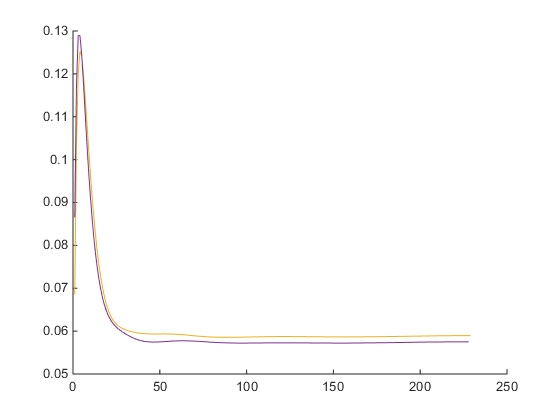
\includegraphics[width=10cm]{TESTimg.png}
 \caption{Test figure for list of figures.}
\label{Cd_mesh_ind}
\end{figure}
 %
%\subsection{Summary}

% TEST

\begin{table}[H]
\caption{Test table for list of tables.}
\centering
\begin{tabular}{lccr}
 & \textbf{Coarse}& \textbf{Fine} & \textbf{Relative difference} \\
Mesh nodes & 251486 & 569727 & 127\% \\
$C_D$ & 0.05896 & 0.057497 & -2.5\% \\
$C_L$ & 1.3541 & 1.3796 & 1.9\% \\
\end{tabular}
\label{meshilainen3dII}
\end{table}

\begin{figure}[H]
 \centering
 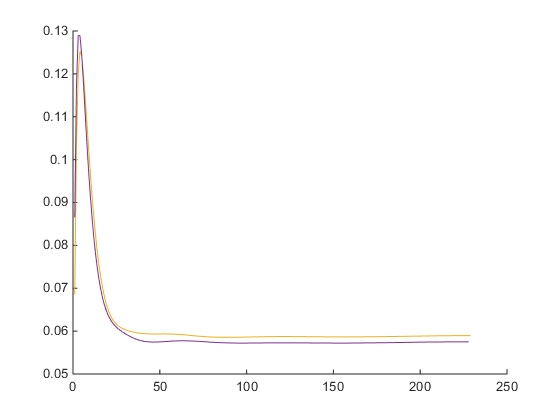
\includegraphics[width=10cm]{TESTimg.png}
 \caption{Test figure for list of figures.}
\label{Cd_mesh_ind}
\end{figure}
 %
         % "CHAPTER" 4
\newpage
\section{Flight Control System}

\subsection{Hardware}
\subsection{Arduino Programming}
                % "CHAPTER" 5
\section{Validation}
         % "CHAPTER" 6
\section{Discussion}
         % "CHAPTER" 7
\section{Summary \& Recommendations}
       % "CHAPTER" 8


\newpage
\bibliographystyle{unsrt}
\nocite{*}
\bibliography{ref}

\end{document}

\pagebreak
\appendix



% %Use Bibtex for references and the \texttt{cite} command to refer to the sources. See the .bbl file. Note - there are more available entries than you find in the file. Add your references as appropriate entries and compile at least three times. Citation: The first is to a web page~\cite{website:Tornado}. The second to a journal paper (article)~\cite{laurence:boundary}, and the third to a book~\cite{blazek:cfd}.


% \section{Matlab Code for NACA 4-digit series airfoil}
% \lstset{columns=fullflexible, basicstyle=\ttfamily}
% Please note that if the resolution $n$ is set too high there might be problems when importing the coordinate file into Workbench Geometry.
% \begin{lstlisting}
% % function[M1,M2] = NACA4digit(NACA,c,n,cut) %Comment NACA,c,n and cut in
% % code if function calling is to be used

% clear all
% close all
% clc

% \end{lstlisting}
